\documentclass[12pt]{article}
% Packages
\usepackage[utf8]{inputenc}
\usepackage{hyperref}
\usepackage[T1]{fontenc}
\usepackage{csvsimple}
\usepackage{datatool}
\usepackage{graphicx}
\graphicspath{ {/home/Users/Theo/dev/porjetMemoire/LateX/} }
% Settings and data
\hypersetup{
    colorlinks=true,
    linkcolor=blue,
    filecolor=magenta,      
    urlcolor=cyan,
    pdftitle={Overleaf Example},
    pdfpagemode=FullScreen,
    }



\title{Rapport sur les travaux de mon memoire}
\author{Theophile Miailhe}
\date{1/04/22}

\begin{document}
\maketitle

\section{Travail accoumpli :}
\paragraph*{}
Grâce à la disponibilité en format CSV de la base de données des morts en opération extérieure, je n'ai pas eu besoin de faire un scrapping du site du SHD. J'ai téléchargé les données directement de ce lien: \url{https://www.memoiredeshommes.sga.defense.gouv.fr/fr/arkotheque/navigation_facette/index.php?f=opendata}. J'ai procédé à un traitement avec de la  base « Militaires décédés sur les théâtres d'opérations extérieurs (1905-1962) » avec Pandas.
La base comportait 20.059 entrées qui correspondaient chacune à un militaire mort.  
\begin{figure}[htp]
    \centering
    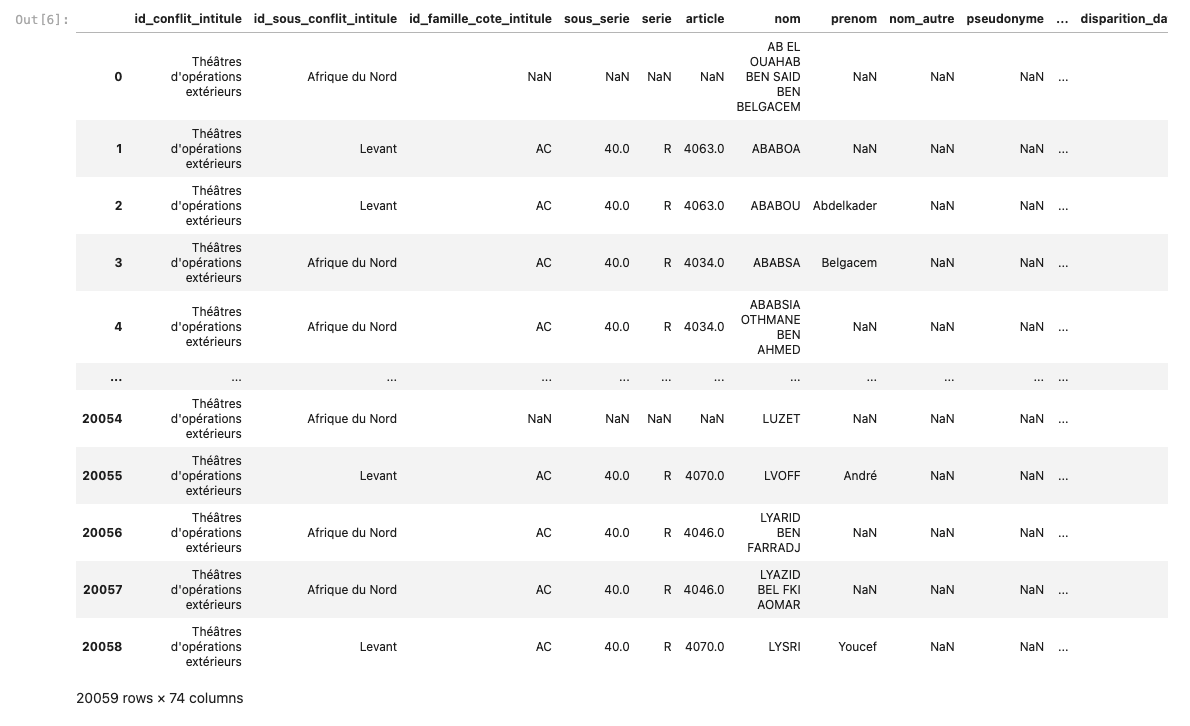
\includegraphics[scale=0.27]{dbpic.png}
    \caption{Base d'origine}
    \label{fig:Base d'origine}
\end{figure}Ensuite j'ai filtré la base par année et par lieu de décès. La période qui m'intéresse est de janvier 1925 à décembre 1926 où la majorité des combats ont eu lieu. Dans la base, il y a une colonne pour le pays de décès et là j'ai filtré pour le Maroc. Le script que j'ai utilisé pour filtrer la base se trouve sur la branch v.02 de mon projet sur \href{https://github.com/the0phil3/projetMemoire/tree/v.02}{Github}. Ce travail m'a permis de créer une base de données de personnelle des sujets qui m'intéressent : 
  



\end{document}